%% Creator: Inkscape inkscape 0.48.5, www.inkscape.org
%% PDF/EPS/PS + LaTeX output extension by Johan Engelen, 2010
%% Accompanies image file 'EvaluationL.pdf' (pdf, eps, ps)
%%
%% To include the image in your LaTeX document, write
%%   \input{<filename>.pdf_tex}
%%  instead of
%%   \includegraphics{<filename>.pdf}
%% To scale the image, write
%%   \def\svgwidth{<desired width>}
%%   \input{<filename>.pdf_tex}
%%  instead of
%%   \includegraphics[width=<desired width>]{<filename>.pdf}
%%
%% Images with a different path to the parent latex file can
%% be accessed with the `import' package (which may need to be
%% installed) using
%%   \usepackage{import}
%% in the preamble, and then including the image with
%%   \import{<path to file>}{<filename>.pdf_tex}
%% Alternatively, one can specify
%%   \graphicspath{{<path to file>/}}
%% 
%% For more information, please see info/svg-inkscape on CTAN:
%%   http://tug.ctan.org/tex-archive/info/svg-inkscape
%%
\begingroup%
  \makeatletter%
  \providecommand\color[2][]{%
    \errmessage{(Inkscape) Color is used for the text in Inkscape, but the package 'color.sty' is not loaded}%
    \renewcommand\color[2][]{}%
  }%
  \providecommand\transparent[1]{%
    \errmessage{(Inkscape) Transparency is used (non-zero) for the text in Inkscape, but the package 'transparent.sty' is not loaded}%
    \renewcommand\transparent[1]{}%
  }%
  \providecommand\rotatebox[2]{#2}%
  \ifx\svgwidth\undefined%
    \setlength{\unitlength}{704bp}%
    \ifx\svgscale\undefined%
      \relax%
    \else%
      \setlength{\unitlength}{\unitlength * \real{\svgscale}}%
    \fi%
  \else%
    \setlength{\unitlength}{\svgwidth}%
  \fi%
  \global\let\svgwidth\undefined%
  \global\let\svgscale\undefined%
  \makeatother%
  \begin{picture}(1,0.27272727)%
    \put(0,0){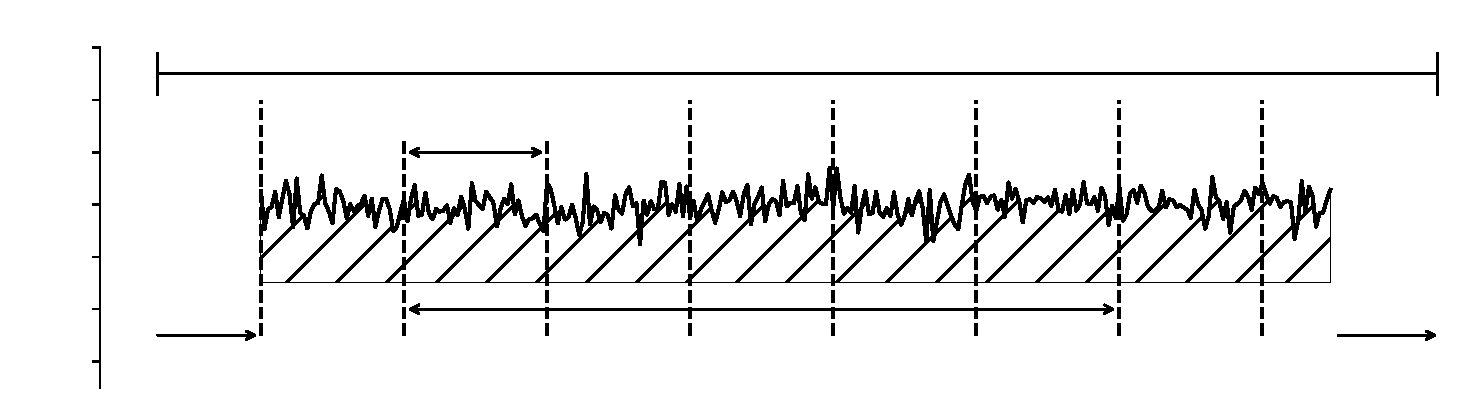
\includegraphics[width=\unitlength]{EvaluationL.pdf}}%
    \put(0.05817717,0.02092365){\makebox(0,0)[rb]{\smash{−4}}}%
    \put(0.05817717,0.05656176){\makebox(0,0)[rb]{\smash{−2}}}%
    \put(0.05817717,0.09219988){\makebox(0,0)[rb]{\smash{0}}}%
    \put(0.05817717,0.12783799){\makebox(0,0)[rb]{\smash{2}}}%
    \put(0.05817717,0.1634761){\makebox(0,0)[rb]{\smash{4}}}%
    \put(0.05817717,0.19911421){\makebox(0,0)[rb]{\smash{6}}}%
    \put(0.05817717,0.23475232){\makebox(0,0)[rb]{\smash{8}}}%
    \put(0.02860065,0.12432508){\rotatebox{90}{\makebox(0,0)[b]{\smash{Heights (a.u.)}}}}%
    \put(0.32419552,0.18669178){\makebox(0,0)[b]{\smash{Sampling lenght}}}%
    \put(0.54368852,0.24014894){\makebox(0,0)[b]{\smash{Transverse length}}}%
    \put(0.51930042,0.02632027){\makebox(0,0)[b]{\smash{Evaluation length (Assesment length)}}}%
    \put(0.14128469,0.06195839){\makebox(0,0)[b]{\smash{Run-up}}}%
    \put(0.94609235,0.06195839){\makebox(0,0)[b]{\smash{Over travel}}}%
  \end{picture}%
\endgroup%
